\section{Introduction}
To effectively navigate the intricacies of software development and guarantee the project's success, choosing an appropriate approach is essential.
The concepts, procedures, and practices that guide a project's development, implementation, and completion are collectively referred to as its methodology.
The variety of alternative methods, each with specific advantages and applicability to various project types, means that selecting a methodology should be done with careful consideration.
This section explores the reasoning behind the choice of an Agile-based methodology, with a particular emphasis on the Kanban methodology, made by the use of Notion for project management.
This decision was driven by the project's requirement for flexibility, continuous improvement, and a visual workflow management system. 
The following sections will outline the comparative comparison between various approaches, along with the reasoning behind choosing Agile due to its alignment with the project's objectives and task specifications.

\section{Research Methodology}
\subsection{Waterfall methodology}
\begin{figure}[!ht]
    \centering
    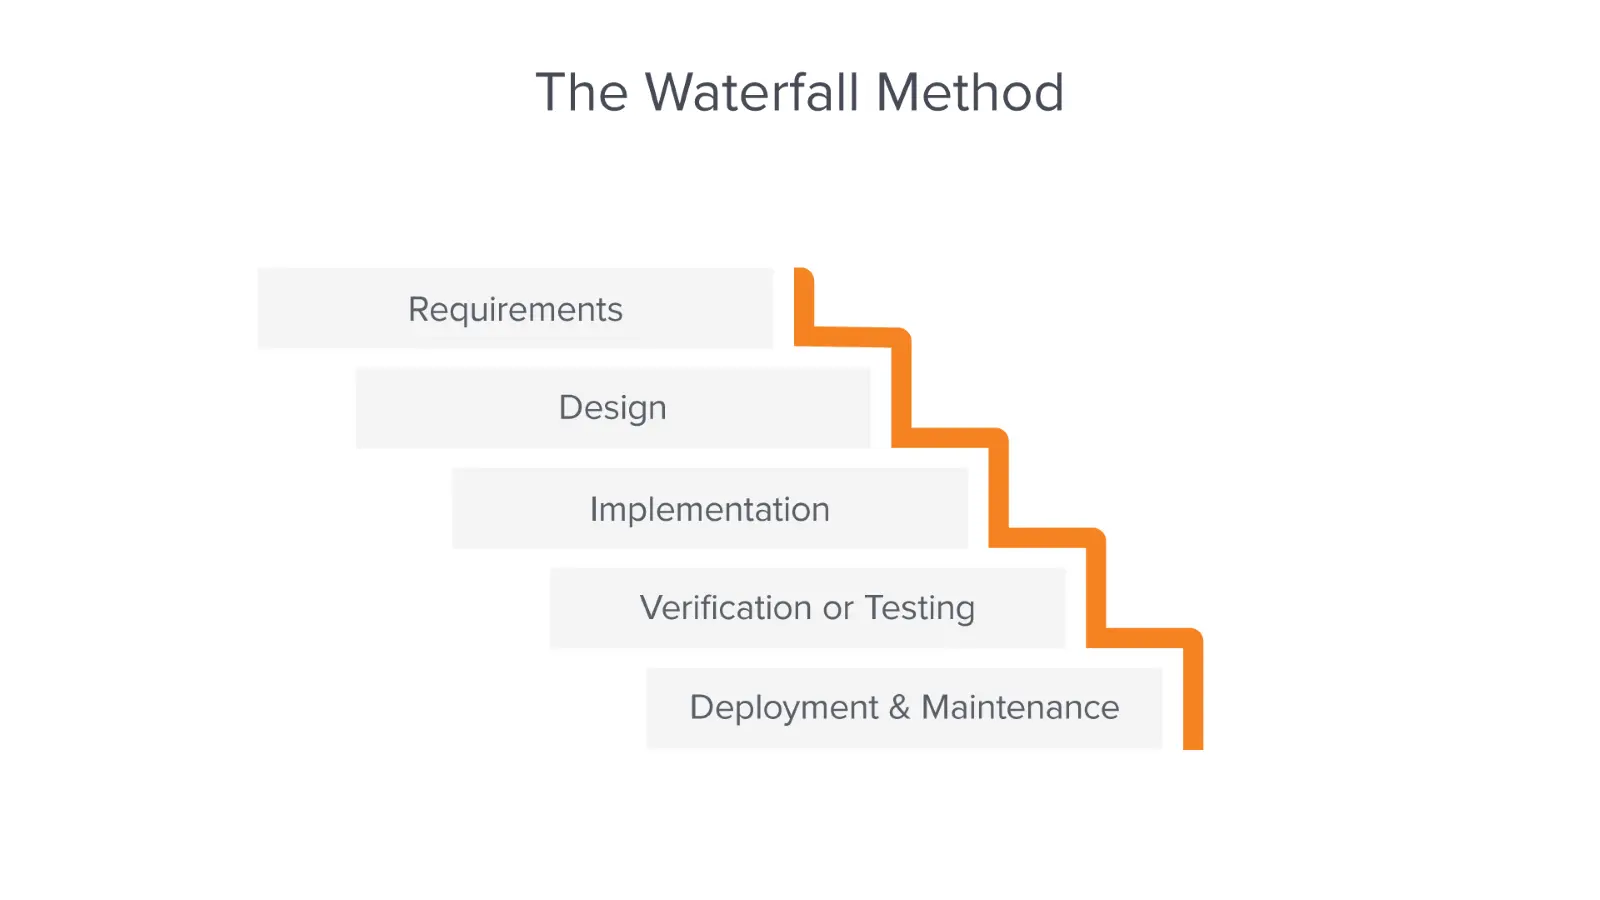
\includegraphics[width=10cm]{Images/watefall.png}
    \caption{Waterfall Methodology \citep{communitcationteam_2022_waterfall}}
    \label{fig:waterfall}
\end{figure}
Waterfall methodology, with its linear and sequential approach, stands as a traditional yet relevant framework for software development projects that require a clear, phased progression.
Requirements, design, implementation, testing, development and maintenance are the steps in this process.
They guarantee that one phase must be finished before moving on to the next, which makes them especially appropriate for projects with stable, well-defined requirements that are unlikely to change.
Crespo-Santiago \& de la Cruz Dávila-Cosme \citep{cresposantiago_2022_waterfall} highlight the Waterfall methodology helps maintain the scope of their library project within the requirements, estabilishing cost and time control, and documenting evidence of project governance.

\subsection{Spiral methodology}
\begin{figure}[!ht]
    \centering
    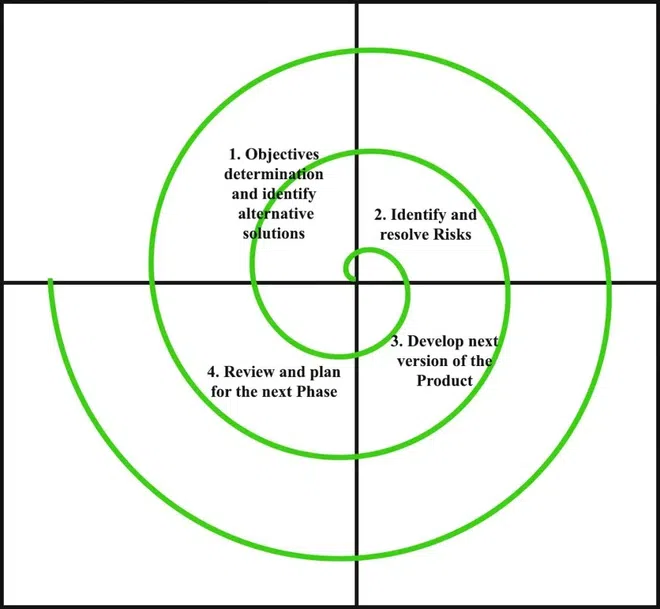
\includegraphics[width=7cm]{Images/spiral.png}
    \caption{Spiral Methodology \citep{kumarpal_2018_software}}
    \label{fig:spiral}
\end{figure}
Spiral methodology, an evolutionary software development process introduced by Barry Boehm in 1986, is a model for process flexibility and risk control in software development. \citep{boehm_1986_a}
The methodology is distinguished by its four-phase cycle approach, which includes planning, risk analysis, implementation, evaluation.
This allows for ongoing iterations that involve setting project goals, identifying potential risks, carrying out development, and incorporating stakeholder feedback.
Its iterative design ensures a flexible and adaptive development process by permitting incremental product improvements based on changing needs and stakeholder input.
The Spiral methodology provides a methodical approach to managing the complexities and uncertainties inherent in software development. 
It shines in contexts where project needs are ambiguous or subject to change because of its heavy emphasis on risk management. 

\subsection{Agile methodology}
\begin{figure}[!ht]
    \centering
    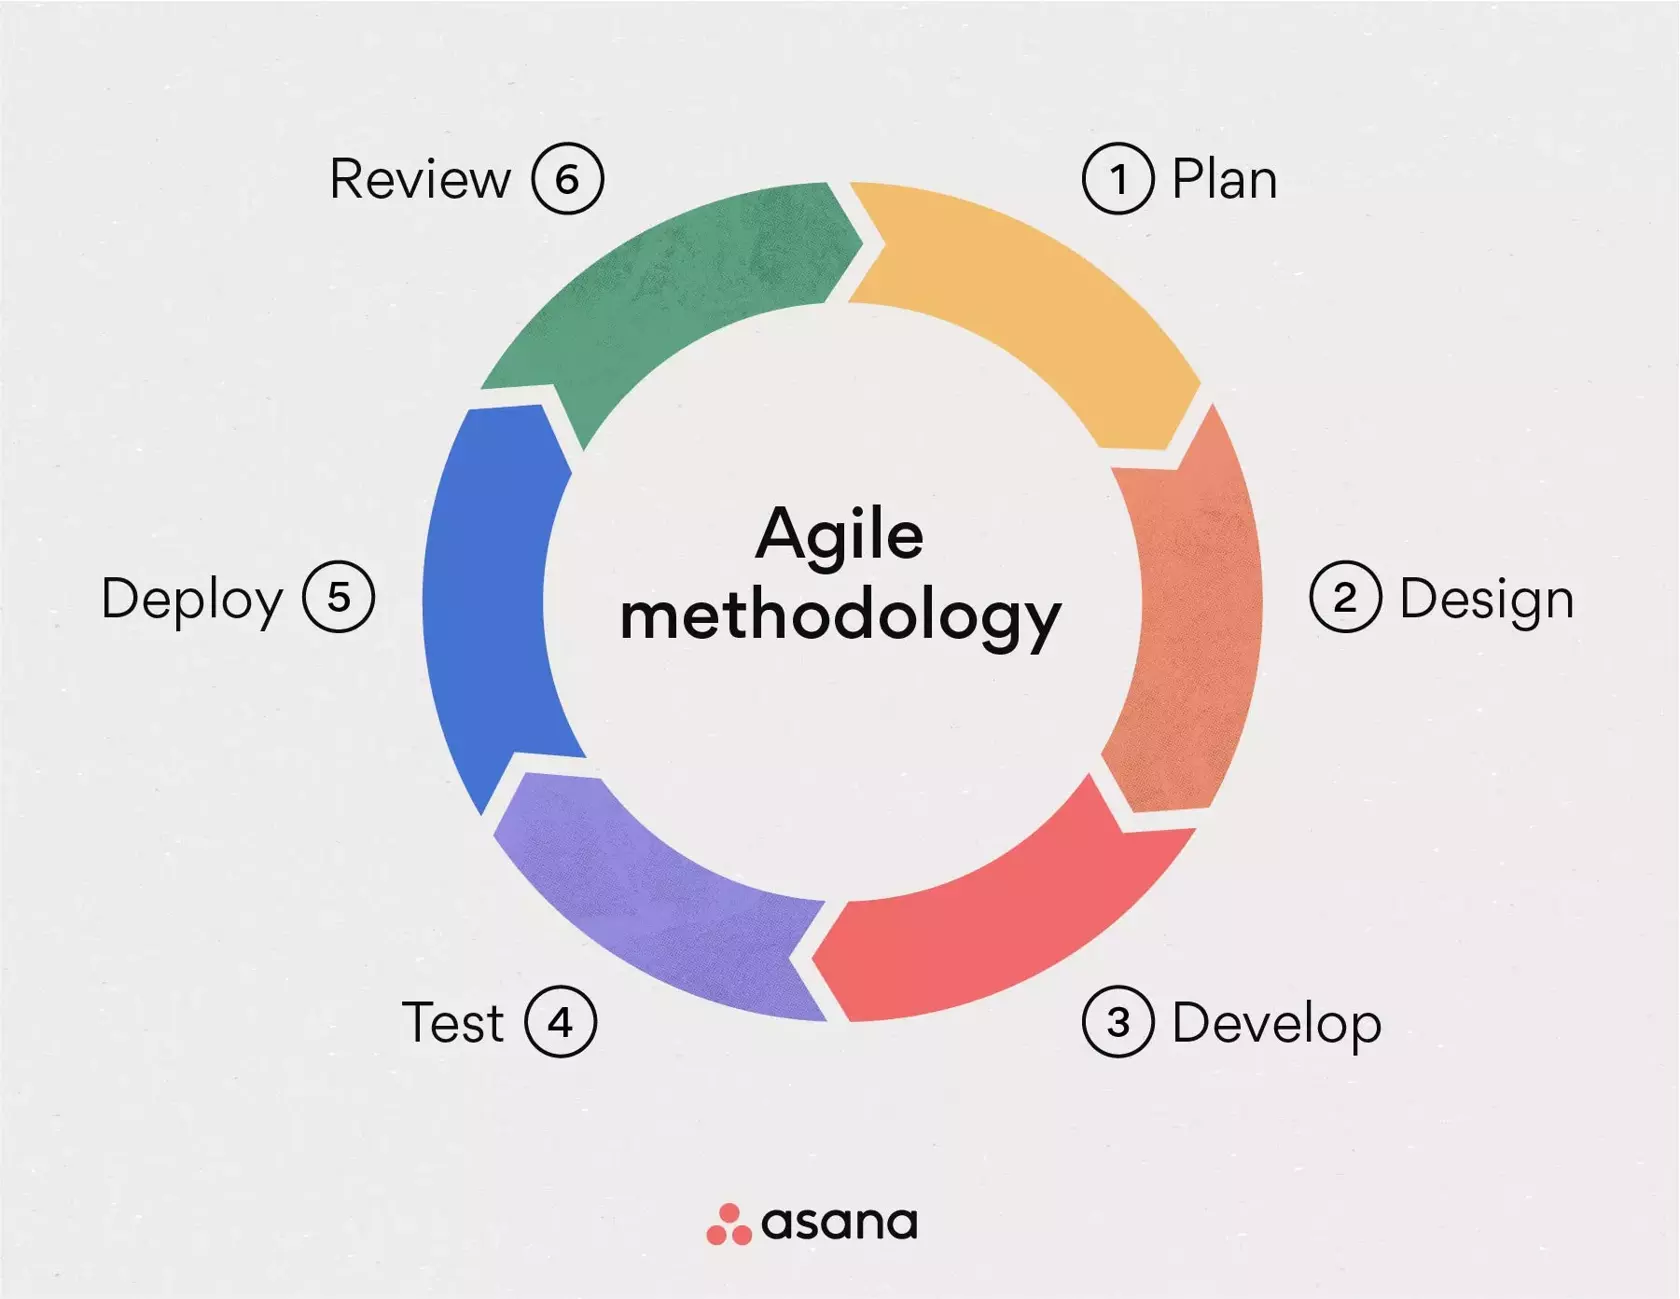
\includegraphics[width=7cm]{Images/agile.png}
    \caption{Agile Methodology \citep{laoyan_2022_what}}
    \label{fig:agile}
\end{figure}
Agile methodology, an approach originated from the Agile Manifesto, published in 2001 by a group of software developers, prioritizes adaptability, collaboration, customer satisfaction and timely delivery of high-quality software.
While implementing Agile methodology, project is breaks into small, manageable pieces, known as iterations or sprints.
Each sprint involves cross-functional teams working on various aspects like planning, design, coding, and testing, with a working iteration of the product delivered at the end of each cycle. 
This methodology works effectively for projects whose requirements are changing or unclear since it allows ongoing feedback and adjustment. 

\section{Comparison and Selection}
\begin{table}[htbp]
    \centering
    \caption{Comparison of Methodologies}
    \label{tab:methodologies}
    \begin{tabularx}{\textwidth}{>{\bfseries}lXXX}
    \toprule
    Aspect & Agile & Waterfall & Spiral \\
    \addlinespace
    Pros & 
    \begin{itemize}
        \item High flexibility and adaptability to changes.
        \item Frequent releases and feedback.
        \item Enhanced customer satisfaction.
        \item Reduced time to market.
    \end{itemize} & 
    \begin{itemize}
        \item Simple and easy to understand and use.
        \item Clear project milestones and deliverables.
        \item Well-suited for projects with defined requirements.
    \end{itemize} & 
    \begin{itemize}
        \item Focus on risk management.
        \item Flexibility in design and development.
        \item Suitable for large, complex projects with uncertain risks.
    \end{itemize} \\
    \addlinespace
    Cons & 
    \begin{itemize}
        \item Less predictable budget and timeline.
        \item Requires close collaboration and customer involvement.
        \item Not ideal for low-change projects or those with fixed requirements.
    \end{itemize} & 
    \begin{itemize}
        \item Difficult to incorporate changes once the project has started.
        \item Potential for late discovery of problems or errors.
        \item Not suitable for projects where requirements may evolve.
    \end{itemize} & 
    \begin{itemize}
        \item Can be complex and costly to implement.
        \item Requires significant risk assessment expertise.
        \item May lead to prolonged project duration due to iterative nature.
    \end{itemize} \\
    \bottomrule
    \end{tabularx}
\end{table}    
Software development can be approached differently using the Agile, Waterfall, and Spiral techniques, each with its own set of benefits and difficulties.
From Table \ref{tab:methodologies}, Agile is highly flexible and adaptable, ideal for projects with evolving requirements, but may lead to unpredictable costs.
Waterfall is straightforward and orderly, perfect for projects with well-defined requirements, but inflexible to changes.
Spiral combines iterative development with focusing on risk management, but it could be costly. 
The project's scale and the clarity of its needs determine which technique is best: Waterfall for its structure, Agile for its flexibility, or Spiral for its risk emphasis.


\section{Justification for Choosing Agile}
The Agile methodology, particularly the Kanban variant, was chosen in order to satisfy the demand for an adaptable, graphical, and iterative developments process.
Given the dynamic nature of the project and its ever-changing objectives, Kanban, which places a strong focus on continuous delivery and workflow efficiency, is an excellent fit.
\\
\begin{figure}[!ht]
    \centering
    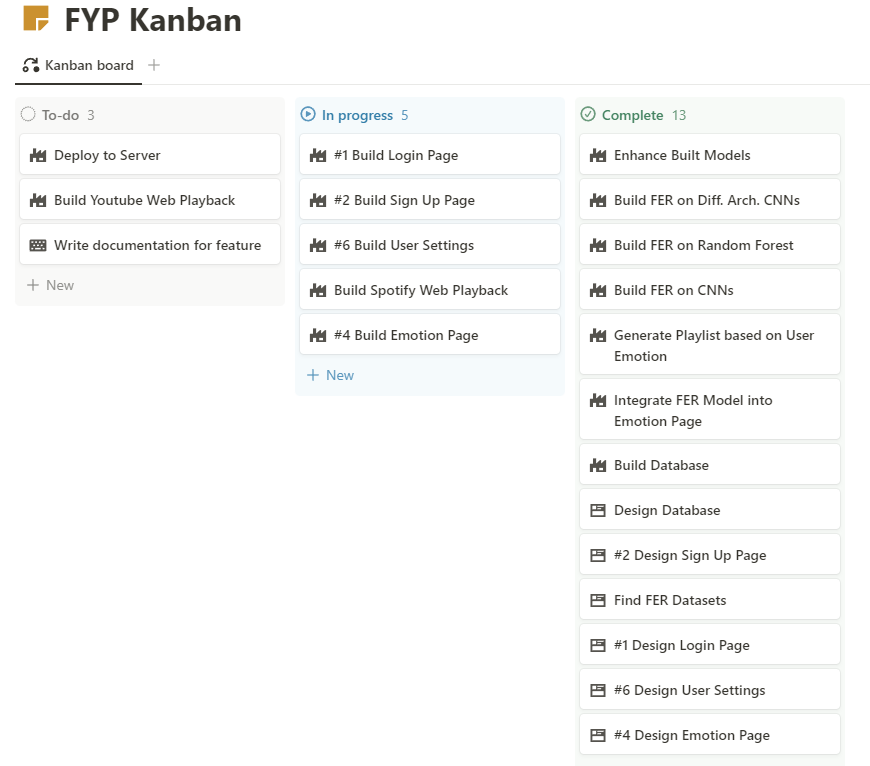
\includegraphics[width=12cm]{Images/kanban.png}
    \caption{Kanban from Notion}
    \label{fig:kanban}
\end{figure}
\\
\indent In this project, Kanban is implementing using Notion. 
It gives tasks a visual representation, making it easier to organize and keep track of them as they go through various stages of development.
Also, with the adaptability of Notion's platform, project plans could be updated easily which is crucial for keeping the plan responsive to changing project dynamics.
\\
\indent Kanban method's inherent simplicity and its focus on delivering work just-in-time are particularly beneficial for projects demanding flexibility and time efficiency.
Kanban with Notion provides a clear picture of the project's progress, enabling developer to identify and resolve bottlenecks quickly, and efficiently manage task prioritization.
Therefore, the combination of Notion's features with Agile Kanban creates a strong foundation for project management by fusing Kanban's visual clarity and streamlined efficiency with Agile's flexibility. 

